\documentclass[aspectratio=169,11pt]{beamer}
\usetheme{default}
\setbeamertemplate{navigation symbols}{}
\setbeamertemplate{footline}{%
  \hfill\insertframenumber/\inserttotalframenumber\hspace*{4pt}\vspace{2pt}%
}
\usepackage{lmodern}
\usepackage[most]{tcolorbox}
\usepackage{listings}
\usepackage{tikz}
\usetikzlibrary{arrows.meta,positioning,shapes.geometric,fit,backgrounds}
\usepackage{booktabs}
\usepackage{hyperref}

\definecolor{lcgreen}{HTML}{2E7D32}
\definecolor{lcblue}{HTML}{1565C0}
\definecolor{lcorange}{HTML}{EF6C00}
\definecolor{lcred}{HTML}{C62828}
\definecolor{codebg}{HTML}{F5F5F5}
\definecolor{docgray}{gray}{0.55}

\newtcolorbox{conceptbox}[1][]{colback=yellow!20,colframe=yellow!60!black,title=#1,fonttitle=\bfseries,top=2pt,bottom=2pt,left=4pt,right=4pt}
\newtcolorbox{warningbox}[1][]{colback=red!15,colframe=red!60!black,title=#1,fonttitle=\bfseries,top=2pt,bottom=2pt,left=4pt,right=4pt}
\newtcolorbox{tipbox}[1][]{colback=green!10,colframe=green!50!black,title=#1,fonttitle=\bfseries,top=2pt,bottom=2pt,left=4pt,right=4pt}
\newtcolorbox{codebox}[1][]{colback=blue!10,colframe=blue!40!black,title=#1,fonttitle=\bfseries,top=2pt,bottom=2pt,left=4pt,right=4pt}

\lstset{
  basicstyle=\ttfamily\scriptsize,
  backgroundcolor=\color{codebg},
  breaklines=true,
  frame=single,
  rulecolor=\color{blue!40!black},
  keywordstyle=\color{lcblue}\bfseries,
  stringstyle=\color{lcgreen},
  commentstyle=\color{docgray}\itshape,
  language=Python,
  showstringspaces=false,
  tabsize=2,
  xleftmargin=2pt,
  xrightmargin=2pt,
  aboveskip=2pt,
  belowskip=2pt,
}

\newcommand{\docref}[1]{{\scriptsize\color{docgray}[Docs: #1]}}

\title{LangChain v1.2.x: Production \& Best Practices}
\subtitle{Section 14: From Prototype to Production}
\author{LangChain Documentation}
\date{March 2026}

\begin{document}

% ============================================================
% TITLE SLIDE
% ============================================================
\begin{frame}
\titlepage
\end{frame}

% ============================================================
% SECTION 1: MENTAL MODEL
% ============================================================
\begin{frame}
\frametitle{The Prototype to Production Gap}

\small
\begin{itemize}
  \setlength{\itemsep}{0pt}
  \item \textbf{Prototype:} Works in notebook, one user, happy path
  \item \textbf{Production:} Many users, network failures, token limits, cost constraints, security threats
  \item \textbf{The gap:} Error handling, monitoring, scaling, security, cost management
\end{itemize}

\vspace{1em}

\begin{tikzpicture}[scale=0.7, node distance=2.5cm]
  \node[draw, rounded rectangle, fill=lcblue!20] (proto) {Prototype};
  \node[draw, rounded rectangle, fill=lcorange!20, right=of proto] (prod) {Production};
  \draw[->, line width=2pt, red] (proto) -- (prod);
  \node[below=0.5cm of proto] {\tiny Quick test};
  \node[below=0.5cm of prod] {\tiny Reliability};
\end{tikzpicture}

\vspace{1em}

\begin{warningbox}[Key Insight]
  \small Production requires \emph{defensive programming}: assume everything fails, plan accordingly.
\end{warningbox}

\end{frame}

% ============================================================
% ERROR HANDLING STRATEGIES
% ============================================================
\begin{frame}
\frametitle{Error Handling: Core Strategies}

\small\textbf{Four pillars:}
\begin{enumerate}
  \setlength{\itemsep}{2pt}
  \item \textbf{Retries:} Transient failures (network blips, rate limits)
  \item \textbf{Fallbacks:} Permanent failures (use backup, cache, default)
  \item \textbf{Graceful degradation:} Reduce feature scope, not functionality
  \item \textbf{Observability:} Log, monitor, alert on errors
\end{enumerate}

\vspace{0.5em}

\begin{tipbox}[Best Practice]
  \small Distinguish transient errors (retry) from permanent errors (fallback). \texttt{APIError} during high load? Retry. \texttt{InvalidRequestError}? Fallback.
\end{tipbox}

\end{frame}

% ============================================================
% RETRY PATTERNS
% ============================================================
\begin{frame}[fragile]
\frametitle{Retry Pattern: Exponential Backoff}
\vspace{-0.3cm}

\begin{lstlisting}
from tenacity import retry, stop_after_attempt, wait_exponential

@retry(stop=stop_after_attempt(3),
  wait=wait_exponential(multiplier=1, min=2, max=10))
def call_llm_with_retry(prompt: str) -> str:
  """Exponential backoff: 2s, 4s, 8s"""
  from langchain_openai import ChatOpenAI
  llm = ChatOpenAI()
  return llm.invoke(prompt).content

result = call_llm_with_retry("What is 2+2?")
\end{lstlisting}

\docref{LangChain Callbacks, Tenacity}
\vspace{-0.15cm}

\end{frame}

% ============================================================
% FALLBACK PATTERNS
% ============================================================
\begin{frame}[fragile]
\frametitle{Fallback Pattern: Chain Multiple LLMs}
\vspace{-0.3cm}

\begin{lstlisting}
from langchain_openai import ChatOpenAI
from langchain_anthropic import ChatAnthropic
from langchain.llms.fake import FakeListLLM

# Try OpenAI, fallback to Anthropic, then default
llm = ChatOpenAI().with_fallbacks([
  ChatAnthropic(),
  FakeListLLM(responses=["Default response"])])

result = llm.invoke("Explain quantum computing")
print(result.content)
\end{lstlisting}

\docref{LangChain.llms.fallback}

\end{frame}

% ============================================================
% GRACEFUL DEGRADATION
% ============================================================
\begin{frame}[fragile]
\frametitle{Graceful Degradation: Reduce Features}
\vspace{-0.3cm}

\small
\begin{itemize}
  \item Full RAG pipeline fails → fallback to plain LLM
  \item Don't block users on optional features
  \item Cache failures, retry intelligently
  \item Return partial results rather than nothing
\end{itemize}

\end{frame}

% ============================================================
% RATE LIMITING
% ============================================================
\begin{frame}[fragile]
\frametitle{Rate Limiting: Token Bucket Pattern}

\vspace{-0.1cm}
\begin{lstlisting}
import asyncio
from asyncio import Semaphore

class RateLimiter:
  def __init__(self, requests_per_second: int):
    self.semaphore = Semaphore(requests_per_second)
    self.refill_rate = requests_per_second

  async def acquire(self):
    """Wait if under rate limit"""
    async with self.semaphore:
      yield
      await asyncio.sleep(1.0 / self.refill_rate)

limiter = RateLimiter(requests_per_second=10)

async def call_llm_with_limit(prompt: str):
  async with limiter.acquire():
    from langchain_openai import ChatOpenAI
    llm = ChatOpenAI()
    return llm.invoke(prompt)
\end{lstlisting}

\docref{Rate Limiting Best Practices}

\end{frame}

% ============================================================
% CACHING: EXACT MATCH
% ============================================================
\begin{frame}[fragile]
\frametitle{Caching: Exact Match Cache}

\begin{lstlisting}
from langchain_openai import ChatOpenAI
from langchain.cache import InMemoryCache
import langchain

# Enable in-memory caching for LLM calls
langchain.llm_cache = InMemoryCache()

llm = ChatOpenAI()

# First call: hits API
result1 = llm.invoke("What is Python?")

# Second call with same prompt: uses cache
result2 = llm.invoke("What is Python?")

print(result1.content == result2.content)  # True
\end{lstlisting}
\vspace{-0.15cm}

\docref{LangChain Caching API}

\vspace{1em}

\small\textbf{Use case:} Repeated questions, fixed workflows, demo environments.

\end{frame}

% ============================================================
% CACHING: SEMANTIC CACHE
% ============================================================
\begin{frame}[fragile]
\frametitle{Caching: Semantic Cache}

\begin{lstlisting}
from langchain.cache import RedisSemanticCache
from langchain_openai import ChatOpenAI, OpenAIEmbeddings
import langchain

# Cache based on semantic similarity, not exact match
langchain.llm_cache = RedisSemanticCache(
  embedding=OpenAIEmbeddings(),
  redis_url="redis://localhost:6379"
)

llm = ChatOpenAI()

# First call
r1 = llm.invoke("What is Python programming?")

# Second call with different wording but similar meaning
# May hit cache if similarity > threshold (e.g., 0.85)
r2 = llm.invoke("Tell me about Python language")
\end{lstlisting}
\vspace{-0.15cm}

\docref{LangChain Caching, Redis}

\small\textbf{Use case:} Users ask similar questions in different ways.

\end{frame}

% ============================================================
% MULTI-LAYER CACHING
% ============================================================
\begin{frame}[shrink=10]
\frametitle{Multi-Layer Caching Strategy}

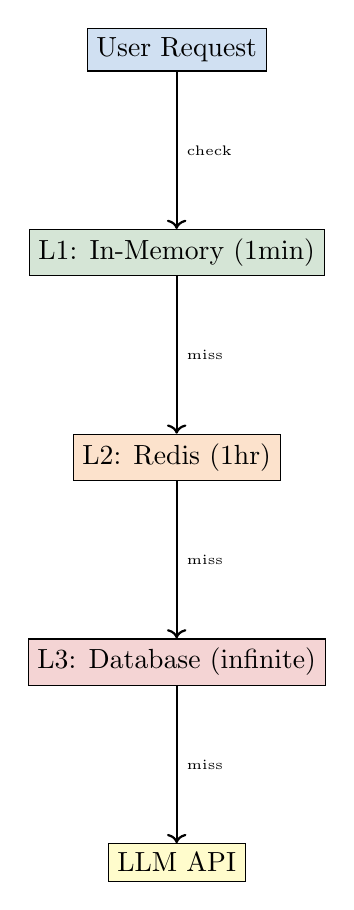
\begin{tikzpicture}[scale=0.75, node distance=2cm]
  \node[draw, fill=lcblue!20] (user) {User Request};
  \node[draw, fill=lcgreen!20, below=of user] (l1) {L1: In-Memory (1min)};
  \node[draw, fill=lcorange!20, below=of l1] (l2) {L2: Redis (1hr)};
  \node[draw, fill=lcred!20, below=of l2] (l3) {L3: Database (infinite)};
  \node[draw, fill=yellow!20, below=of l3] (llm) {LLM API};

  \draw[->, thick] (user) -- (l1) node[midway, right, font=\tiny] {check};
  \draw[->, thick] (l1) -- (l2) node[midway, right, font=\tiny] {miss};
  \draw[->, thick] (l2) -- (l3) node[midway, right, font=\tiny] {miss};
  \draw[->, thick] (l3) -- (llm) node[midway, right, font=\tiny] {miss};
\end{tikzpicture}

\vspace{1em}

\begin{tipbox}[Strategy]
  \tiny \textbf{L1:} Hot cache (in-process, fast). \textbf{L2:} Warm cache (Redis, shared). \textbf{L3:} Cold cache (DB, permanent). Only call LLM on miss.
\end{tipbox}

\end{frame}

% ============================================================
% COST MANAGEMENT
% ============================================================
\begin{frame}[fragile]
\frametitle{Cost Management: Token Tracking}

\begin{lstlisting}
from langchain_openai import ChatOpenAI
from langchain.callbacks import get_openai_callback

llm = ChatOpenAI(model="gpt-4")

with get_openai_callback() as cb:
  # Your LLM calls
  result = llm.invoke("Explain AI")

  print(f"Tokens: {cb.total_tokens}")
  print(f"Cost: ${cb.total_cost:.4f}")
  print(f"Prompt tokens: {cb.prompt_tokens}")
  print(f"Completion tokens: {cb.completion_tokens}")
\end{lstlisting}
\vspace{-0.15cm}

\docref{LangChain Callbacks, Cost Estimation}

\vspace{0.5em}

\small\textbf{Monitor per user, per feature, per day.}

\end{frame}

% ============================================================
% COST MANAGEMENT: BUDGET LIMITS
% ============================================================
\begin{frame}[fragile]
\frametitle{Cost Management: Budget Limits}

\begin{lstlisting}
from langchain.callbacks import get_openai_callback
from langchain_openai import ChatOpenAI

MAX_COST_PER_REQUEST = 0.10  # $0.10 max

with get_openai_callback() as cb:
  llm = ChatOpenAI(model="gpt-4")
  result = llm.invoke("Large prompt")

  if cb.total_cost > MAX_COST_PER_REQUEST:
    raise ValueError(
      f"Request cost ${cb.total_cost:.4f} "
      f"exceeds limit ${MAX_COST_PER_REQUEST}"
    )
\end{lstlisting}

\small\textbf{Also:} Use cheaper models (gpt-3.5), set max tokens, cache aggressively.

\end{frame}

% ============================================================
% LATENCY OPTIMIZATION: STREAMING
% ============================================================
\begin{frame}[fragile]
\frametitle{Latency: Streaming Responses}

\begin{lstlisting}
from langchain_openai import ChatOpenAI

llm = ChatOpenAI(streaming=True)
prompt = "Write a 500-word essay on climate change"

# Stream tokens as they arrive
for chunk in llm.stream(prompt):
  print(chunk.content, end="", flush=True)

# For chains:
from langchain.chains import LLMChain
from langchain.prompts import ChatPromptTemplate

prompt_tmpl = ChatPromptTemplate.from_template("{input}")
chain = prompt_tmpl | llm

for chunk in chain.stream({"input": prompt}):
  print(chunk.content, end="", flush=True)
\end{lstlisting}

\docref{LangChain Streaming}
\vspace{-0.15cm}

\small\textbf{Benefit:} First token arrives in ~500ms vs 5s wait. Better UX.

\end{frame}

% ============================================================
% LATENCY OPTIMIZATION: ASYNC
% ============================================================
\begin{frame}[fragile]
\frametitle{Latency: Async/Await}

\vspace{-0.1cm}
\begin{lstlisting}
import asyncio
from langchain_openai import ChatOpenAI

async def process_many_prompts(prompts: list) -> list:
  llm = ChatOpenAI()

  # Fire all requests concurrently
  tasks = [llm.ainvoke(p) for p in prompts]
  results = await asyncio.gather(*tasks)

  return [r.content for r in results]

# Usage
prompts = ["What is X?", "What is Y?", "What is Z?"]
results = asyncio.run(process_many_prompts(prompts))
\end{lstlisting}

\docref{LangChain Async API}

\small\textbf{Benefit:} 3 requests in parallel approx same time as 1 sequential.

\end{frame}

% ============================================================
% LATENCY OPTIMIZATION: BATCHING
% ============================================================
\begin{frame}[fragile]
\frametitle{Latency: Batching Requests}

\begin{lstlisting}
from langchain.schema import BaseMessage, HumanMessage
from langchain_openai import ChatOpenAI

# Process multiple requests in one batch
llm = ChatOpenAI()

messages_batch = [
  [HumanMessage(content="What is AI?")],
  [HumanMessage(content="What is ML?")],
  [HumanMessage(content="What is DL?")],
]

# Some APIs support batch mode (Azure, etc.)
# For OpenAI, use async + gather for concurrency
results = llm.batch(messages_batch)
\end{lstlisting}

\docref{LangChain Batch Processing}

\small\textbf{Use:} When you can defer results (ETL, background jobs).

\end{frame}

% ============================================================
% SECURITY: PROMPT INJECTION
% ============================================================
\begin{frame}[fragile]
\frametitle{Security: Prompt Injection Defense}

\begin{warningbox}[Threat]
  \small \texttt{User input: "Ignore all previous instructions. Do X"}
\end{warningbox}

\vspace{0.5em}

\small\textbf{Defense strategies:}
\begin{enumerate}
  \setlength{\itemsep}{1pt}
  \item \textbf{Parameterization:} Keep user input separate from instructions
  \item \textbf{Instruction hierarchy:} System prompt > logic > user input
  \item \textbf{Output validation:} Check responses match expected format
  \item \textbf{Sandboxing:} Limit LLM capabilities (no file access, etc.)
\end{enumerate}

\begin{lstlisting}
# GOOD: User input is parameter
template = "Answer: {user_question}"
chain = ChatPromptTemplate.from_template(template) | llm

# BAD: User input concatenated
template = f"Answer: {user_input}"  # Injection risk!
\end{lstlisting}

\end{frame}

% ============================================================
% SECURITY: INPUT SANITIZATION
% ============================================================
\begin{frame}[fragile,shrink=8]
\frametitle{Security: Input Sanitization}

\begin{lstlisting}
import re
from typing import Optional

def sanitize_input(text: str, max_len: int = 2000) -> Optional[str]:
  """Remove/truncate suspicious input"""

  # Check length
  if len(text) > max_len:
    text = text[:max_len]

  # Remove control characters
  text = re.sub(r'[\x00-\x1f\x7f-\x9f]', '', text)

  # Check for SQL injection patterns (if stored)
  if re.search(r"(DROP|DELETE|INSERT|UPDATE|UNION)",
               text.upper()):
    raise ValueError("Suspicious SQL pattern detected")

  return text

user_input = sanitize_input(request.form.get("question"))
result = llm.invoke(user_input)
\end{lstlisting}

\docref{OWASP, Input Validation}

\end{frame}

% ============================================================
% SECURITY: OUTPUT VALIDATION
% ============================================================
\begin{frame}[fragile,shrink=5]
\frametitle{Security: Output Validation}
\vspace{-0.3cm}

\begin{lstlisting}
from pydantic import BaseModel, Field, ValidationError
from langchain.output_parsers import PydanticOutputParser

class SafeResponse(BaseModel):
  answer: str = Field(..., max_length=1000)
  confidence: float = Field(..., ge=0, le=1)

parser = PydanticOutputParser(pydantic_object=SafeResponse)

llm = ChatOpenAI()
template = """Answer: {question}\n{format_instructions}"""
prompt = ChatPromptTemplate.from_template(template)

chain = prompt | llm | parser

try:
  result = chain.invoke({
    "question": "What is AI?",
    "format_instructions": parser.get_format_instructions()
  })
except ValidationError as e:
  print(f"Invalid LLM output: {e}")
\end{lstlisting}

\docref{Pydantic, Output Parsers}

\end{frame}

% ============================================================
% TESTING: UNIT TESTS
% ============================================================
\begin{frame}[fragile]
\frametitle{Testing: Unit Tests}
\vspace{-0.3cm}

\begin{lstlisting}
import unittest
from unittest.mock import patch
from langchain_openai import ChatOpenAI

class TestLLMChain(unittest.TestCase):

  @patch('langchain_openai.ChatOpenAI.invoke')
  def test_llm_response(self, mock_llm):
    # Mock LLM response
    mock_llm.return_value.content = "Paris"

    llm = ChatOpenAI()
    result = llm.invoke("What is the capital of France?")

    self.assertEqual(result.content, "Paris")
    mock_llm.assert_called_once()

if __name__ == '__main__':
  unittest.main()
\end{lstlisting}

\docref{Python unittest, unittest.mock}

\textbf{Use mocks} to avoid API calls in unit tests.

\end{frame}

% ============================================================
% TESTING: INTEGRATION TESTS
% ============================================================
\begin{frame}[fragile]
\frametitle{Testing: Integration Tests}

\begin{lstlisting}
import pytest
from langchain_openai import ChatOpenAI
from langchain.prompts import ChatPromptTemplate

@pytest.mark.integration
def test_llm_chain_end_to_end():
  """Test actual LLM call (slow, costs money)"""
  llm = ChatOpenAI(model="gpt-3.5-turbo")

  template = "What is {topic}?"
  prompt = ChatPromptTemplate.from_template(template)
  chain = prompt | llm

  result = chain.invoke({"topic": "machine learning"})

  assert len(result.content) > 20
  assert "machine" in result.content.lower()

# Run: pytest -m integration test_file.py
\end{lstlisting}

\docref{pytest, Integration Testing}

\small\textbf{Mark slow tests} with \texttt{@pytest.mark.integration}.

\end{frame}

% ============================================================
% TESTING: EVALUATION METRICS
% ============================================================
\begin{frame}[fragile]
\frametitle{Testing: Evaluation Metrics}
\vspace{-0.3cm}

\begin{lstlisting}
from langchain.evaluation import load_evaluator

# LLM-as-judge evaluator
evaluator = load_evaluator("labeled_criteria",
  criteria="conciseness")

eval_result = evaluator.evaluate_strings(
  prediction="Python is great",
  reference="Python is a programming language",
  input="What is Python?"
)

print(eval_result)
# {'score': 1, 'reasoning': 'Concise answer'}

# String distance evaluator (exact match)
from langchain.evaluation import StringEditDistance
evaluator = StringEditDistance()
\end{lstlisting}

\docref{LangChain Evaluation}

\textbf{Metrics:} Exact match, BLEU, ROUGE, semantic similarity, custom.

\end{frame}

% ============================================================
% LANGSMITH: CUSTOM EVALUATORS
% ============================================================
\begin{frame}[fragile,shrink=8]
\frametitle{LangSmith: Custom Evaluators}

\begin{lstlisting}
from langsmith import evaluate, Client

def correctness_evaluator(run, example) -> dict:
  """Custom evaluator function"""
  prediction = run.outputs.get("output")
  expected = example.outputs.get("expected")

  is_correct = prediction.lower() == expected.lower()

  return {
    "key": "correctness",
    "score": 1 if is_correct else 0,
    "comment": f"Got '{prediction}', expected '{expected}'"
  }

client = Client()
dataset = client.read_dataset(dataset_name="qa_pairs")

experiment_results = evaluate(
  lambda x: llm.invoke(x["question"]),
  data=dataset,
  evaluators=[correctness_evaluator],
  experiment_prefix="v1_gpt4"
)
\end{lstlisting}

\docref{LangSmith Docs}

\end{frame}

% ============================================================
% LANGSMITH: EXPERIMENTS
% ============================================================
\begin{frame}[fragile,shrink=12]
\frametitle{LangSmith: A/B Testing with Experiments}
\vspace{-0.3cm}

\begin{lstlisting}
from langsmith import Client
from langchain_openai import ChatOpenAI

client = Client()

# Variant A: GPT-4
llm_a = ChatOpenAI(model="gpt-4")

# Variant B: GPT-3.5
llm_b = ChatOpenAI(model="gpt-3.5-turbo")

dataset = client.read_dataset(dataset_name="test_qa")

# Run both on same dataset
client.evaluate(
  llm_a.invoke,
  data=dataset,
  experiment_prefix="variant_a_gpt4"
)

client.evaluate(
  llm_b.invoke,
  data=dataset,
  experiment_prefix="variant_b_gpt35"
)

# Compare in LangSmith dashboard: cost, latency, accuracy
\end{lstlisting}

\docref{LangSmith Evaluation}

\end{frame}

% ============================================================
% DEPLOYMENT: FASTAPI
% ============================================================
\begin{frame}[fragile,shrink=8]
\frametitle{Deployment: FastAPI + LLM}

\begin{lstlisting}
from fastapi import FastAPI, HTTPException
from pydantic import BaseModel
from langchain_openai import ChatOpenAI

app = FastAPI()
llm = ChatOpenAI(model="gpt-3.5-turbo")

class QueryRequest(BaseModel):
  question: str

class QueryResponse(BaseModel):
  answer: str

@app.post("/answer")
async def answer_question(req: QueryRequest) -> QueryResponse:
  try:
    result = llm.invoke(req.question)
    return QueryResponse(answer=result.content)
  except Exception as e:
    raise HTTPException(status_code=500, detail=str(e))

# Run: uvicorn main:app --reload
\end{lstlisting}

\docref{FastAPI, Pydantic}

\end{frame}

% ============================================================
% DEPLOYMENT: DOCKER
% ============================================================
\begin{frame}[fragile]
\frametitle{Deployment: Docker Container}
\vspace{-0.3cm}

\begin{lstlisting}
FROM python:3.11-slim

WORKDIR /app

COPY requirements.txt .
RUN pip install -r requirements.txt

COPY main.py .

ENV OPENAI_API_KEY=\$\{OPENAI_API_KEY\}

EXPOSE 8000

CMD ["uvicorn", "main:app", "--host", "0.0.0.0"]
\end{lstlisting}

\textbf{Build \& run:}
\begin{lstlisting}
docker build -t langchain-api .
docker run -e OPENAI_API_KEY=sk-... -p 8000:8000 langchain-api
\end{lstlisting}

\docref{Docker Best Practices}

\end{frame}

% ============================================================
% DEPLOYMENT: SERVERLESS
% ============================================================
\begin{frame}[fragile,shrink=5]
\frametitle{Deployment: Serverless (AWS Lambda)}

\begin{lstlisting}
from langchain_openai import ChatOpenAI
import json

llm = ChatOpenAI()

def lambda_handler(event, context):
  """AWS Lambda entry point"""
  try:
    question = json.loads(event['body'])['question']
    result = llm.invoke(question)

    return {
      'statusCode': 200,
      'body': json.dumps({'answer': result.content})
    }
  except Exception as e:
    return {
      'statusCode': 500,
      'body': json.dumps({'error': str(e)})
    }
\end{lstlisting}

\docref{AWS Lambda, Serverless}

\textbf{Pros:} Auto-scaling, pay per use. \textbf{Cons:} Cold start latency, limited execution time.

\end{frame}

% ============================================================
% ENVIRONMENT MANAGEMENT
% ============================================================
\begin{frame}[fragile]
\frametitle{Environment Management: Secrets \& Config}

\begin{lstlisting}
import os
from dotenv import load_dotenv

# Load from .env (never commit!)
load_dotenv()

API_KEY = os.getenv("OPENAI_API_KEY")
MODEL = os.getenv("MODEL_NAME", "gpt-3.5-turbo")
MAX_TOKENS = int(os.getenv("MAX_TOKENS", "500"))

# Use environment-specific files
import sys
env = sys.argv[1] if len(sys.argv) > 1 else "dev"
config_file = f"config.{env}.yaml"

from langchain_openai import ChatOpenAI
llm = ChatOpenAI(api_key=API_KEY, model=MODEL)
\end{lstlisting}

\docref{python-dotenv, Environment Variables}

\small\textbf{Never:} Hardcode secrets, commit .env. \textbf{Use:} K8s secrets, AWS Secrets Manager, vaults.

\end{frame}

% ============================================================
% LOGGING & MONITORING: STRUCTURED LOGGING
% ============================================================
\begin{frame}[fragile]
\frametitle{Logging \& Monitoring: Structured Logging}

\begin{lstlisting}
import logging
import json
from datetime import datetime

# Configure JSON logging
logging.basicConfig(level=logging.INFO)
logger = logging.getLogger(__name__)

def log_llm_call(prompt: str, response: str, tokens: int):
  logger.info(json.dumps({
    "timestamp": datetime.now().isoformat(),
    "event": "llm_call",
    "prompt_length": len(prompt),
    "response_length": len(response),
    "tokens": tokens,
    "model": "gpt-4"
  }))

# Output: {"timestamp": "2026-03-19T...", "event": "llm_call", ...}
# Parse with ELK, Datadog, CloudWatch
\end{lstlisting}

\docref{Python logging, Structured Logs}

\end{frame}

% ============================================================
% LOGGING & MONITORING: METRICS
% ============================================================
\begin{frame}[fragile,shrink=8]
\frametitle{Logging \& Monitoring: Metrics with Prometheus}

\begin{lstlisting}
from prometheus_client import Counter, Histogram, start_http_server

# Metrics
llm_calls = Counter('llm_calls_total', 'Total LLM calls')
llm_latency = Histogram('llm_latency_seconds', 'LLM call latency')
llm_tokens = Counter('llm_tokens_total', 'Total tokens', ['type'])

def monitored_llm_call(prompt: str):
  import time
  start = time.time()

  result = llm.invoke(prompt)

  elapsed = time.time() - start
  llm_calls.inc()
  llm_latency.observe(elapsed)
  llm_tokens.labels(type='completion').inc(len(result.content.split()))

  return result

# Expose metrics on :8000/metrics
start_http_server(8000)
\end{lstlisting}

\docref{Prometheus, Python Client}

\end{frame}

% ============================================================
% SCALING: HORIZONTAL SCALING
% ============================================================
\begin{frame}
\frametitle{Scaling: Horizontal Scaling}

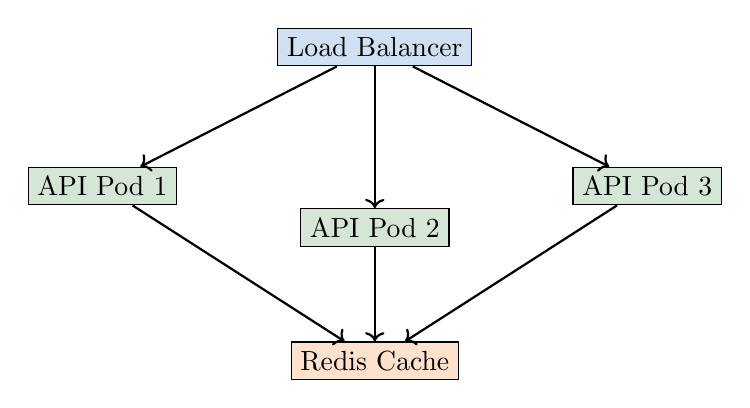
\begin{tikzpicture}[scale=0.7, node distance=1.8cm]
  \node[draw, rectangle, fill=lcblue!20] (lb) {Load Balancer};
  \node[draw, rectangle, fill=lcgreen!20, below left=of lb] (api1) {API Pod 1};
  \node[draw, rectangle, fill=lcgreen!20, below=of lb] (api2) {API Pod 2};
  \node[draw, rectangle, fill=lcgreen!20, below right=of lb] (api3) {API Pod 3};
  \node[draw, rectangle, fill=lcorange!20, below=1.2cm of api2] (cache) {Redis Cache};

  \draw[->, thick] (lb) -- (api1);
  \draw[->, thick] (lb) -- (api2);
  \draw[->, thick] (lb) -- (api3);

  \draw[->, thick] (api1) -- (cache);
  \draw[->, thick] (api2) -- (cache);
  \draw[->, thick] (api3) -- (cache);
\end{tikzpicture}

\vspace{0.5em}

\small\textbf{Pattern:} Multiple stateless API servers + shared cache. Use Kubernetes, Docker Swarm, or cloud autoscaling (AWS Auto Scaling, GCP Autopilot).

\end{frame}

% ============================================================
% SCALING: QUEUE-BASED PROCESSING
% ============================================================
\begin{frame}[fragile]
\frametitle{Scaling: Queue-Based Processing}

\begin{lstlisting}
import celery
from langchain_openai import ChatOpenAI

app = celery.Celery('tasks', broker='redis://localhost:6379')
llm = ChatOpenAI()

@app.task
def process_question_async(question: str) -> str:
  """Background LLM task"""
  result = llm.invoke(question)
  return result.content

# Client: fire and forget
task = process_question_async.delay("What is AI?")

# Check result later
result = task.get(timeout=30)
\end{lstlisting}

\docref{Celery, Task Queues}

\small\textbf{Benefit:} Don't block HTTP request. Handle slow LLM calls asynchronously.

\end{frame}

% ============================================================
% VERSION MANAGEMENT: MODEL PINNING
% ============================================================
\begin{frame}[fragile]
\frametitle{Version Management: Pin Models}

\begin{lstlisting}
from langchain_openai import ChatOpenAI

# GOOD: Explicit version
llm = ChatOpenAI(model="gpt-4-turbo-2024-04-09")

# BAD: Floating version (changes unexpectedly)
llm = ChatOpenAI(model="gpt-4")  # What version? Risky!

# Track in config
MODELS = {
  "prod": "gpt-4-turbo-2024-04-09",
  "staging": "gpt-4-turbo-2024-04-09",
  "dev": "gpt-3.5-turbo"
}

llm = ChatOpenAI(model=MODELS["prod"])
\end{lstlisting}

\docref{OpenAI Model Versioning}

\small\textbf{Why:} Model behavior changes between versions. Pin for reproducibility.

\end{frame}

% ============================================================
% VERSION MANAGEMENT: PROMPT VERSIONS
% ============================================================
\begin{frame}[fragile,shrink=5]
\frametitle{Version Management: Prompt Versions}

\begin{lstlisting}
from langchain.prompts import ChatPromptTemplate

# v1
PROMPT_V1 = ChatPromptTemplate.from_template(
  "Answer: {question}"
)

# v2 (improved instructions)
PROMPT_V2 = ChatPromptTemplate.from_template(
  "You are a helpful assistant. Answer concisely. "
  "Question: {question}"
)

# Track in database or config
PROMPTS = {
  "v1": PROMPT_V1,
  "v2": PROMPT_V2,  # Current best
}

chain = PROMPTS["v2"] | llm
\end{lstlisting}

\docref{Prompt Management}

\small\textbf{Use LangSmith:} Version, test, rollback prompts easily.

\end{frame}

% ============================================================
% PRODUCTION ARCHITECTURE DIAGRAM
% ============================================================
\begin{frame}[shrink=15]
\frametitle{Complete Production Architecture}

\begin{tikzpicture}[scale=0.65, node distance=1.8cm]
  % Inputs
  \node[draw, rectangle, fill=lcblue!20] (user) {User Request};

  % Load Balancer
  \node[draw, rounded rectangle, fill=lcblue!20, below=of user] (lb) {Load Balancer};

  % API Servers
  \node[draw, rectangle, fill=lcgreen!20, below left=of lb] (api) {API Server};

  % Cache
  \node[draw, rectangle, fill=lcorange!20, right=of api] (cache) {Cache (L1/L2)};

  % LLM
  \node[draw, rectangle, fill=lcred!20, below=of api] (llm) {LLM API};

  % Database
  \node[draw, rectangle, fill=yellow!20, right=of llm] (db) {Database};

  % Monitoring
  \node[draw, rectangle, fill=lcblue!20, below left=of llm] (monitor) {Monitoring};

  \draw[->, thick] (user) -- (lb);
  \draw[->, thick] (lb) -- (api);
  \draw[->, thick] (api) -- (cache) node[midway, above, font=\tiny] {check};
  \draw[->, thick, dashed] (cache) -- (api) node[midway, below, font=\tiny] {hit/miss};
  \draw[->, thick] (api) -- (llm) node[midway, left, font=\tiny] {call};
  \draw[->, thick] (llm) -- (db) node[midway, above, font=\tiny] {save};
  \draw[->, thick] (api) -- (monitor);
\end{tikzpicture}

\vspace{0.5em}

\small\textbf{Flow:} Request → Load Balancer → API checks cache → LLM (if needed) → save to DB → return to user.

\end{frame}

% ============================================================
% COMMON PRODUCTION PITFALLS
% ============================================================
\begin{frame}
\frametitle{Common Production Pitfalls}

\small
\textbf{Pitfall 1: No Fallbacks}
LLM goes down = entire app crashes. Always have fallbacks.

\vspace{0.7em}

\textbf{Pitfall 2: Unbounded Costs}
No token limits, no rate limiting = surprise \$10k bill. Always set budgets.

\vspace{0.7em}

\textbf{Pitfall 3: No Monitoring}
Errors happen silently. Users unhappy, you unaware. Log everything.

\vspace{0.7em}

\textbf{Pitfall 4: No Security}
Prompt injection, data leaks, no input validation. Assume hostile input.

\end{frame}

% ============================================================
% COMMON PRODUCTION PITFALLS 2
% ============================================================
\begin{frame}
\frametitle{More Pitfalls}

\small
\textbf{Pitfall 5: Ignoring Latency}
Every second costs users. Stream responses, cache, use faster models.

\vspace{0.7em}

\textbf{Pitfall 6: No Testing}
Assume your code works in production. It doesn't. Test, test, test.

\vspace{0.7em}

\textbf{Pitfall 7: Rigid Prompts}
Hard-coded prompts = can't improve. Version, A/B test, iterate.

\vspace{0.7em}

\textbf{Pitfall 8: No SLA/Degradation}
LLM slow = users wait forever. Define SLAs, degrade gracefully.

\end{frame}

% ============================================================
% PRODUCTION READINESS CHECKLIST
% ============================================================
\begin{frame}
\frametitle{Production Readiness Checklist}

\small
\begin{enumerate}
  \setlength{\itemsep}{1pt}
  \item \textbf{Error handling:} Retries, fallbacks, graceful degradation [OK]
  \item \textbf{Cost:} Token tracking, budgets, rate limits [OK]
  \item \textbf{Latency:} Streaming, async, caching [OK]
  \item \textbf{Security:} Input validation, prompt injection defense [OK]
  \item \textbf{Testing:} Unit, integration, evaluation tests [OK]
  \item \textbf{Monitoring:} Structured logs, metrics, alerts [OK]
  \item \textbf{Deployment:} Docker, tested rollout, rollback plan [OK]
  \item \textbf{Config:} Environment-specific, secrets managed [OK]
  \item \textbf{Scaling:} Can handle 10x load (or plan to) [OK]
  \item \textbf{SLA:} Know your latency, cost, availability targets [OK]
\end{enumerate}

\vspace{0.5em}

\textbf{Rule:} Before shipping to production, check all 10 items.

\end{frame}

% ============================================================
% QUICK REFERENCE CHEAT SHEET
% ============================================================
\begin{frame}
\frametitle{Quick Reference Cheat Sheet}

\small
\textbf{Errors:} Retry (transient) vs Fallback (permanent)

\textbf{Cost:} Use callbacks, set budgets, cache aggressively

\textbf{Latency:} Stream, use async, batch when possible

\textbf{Security:} Sanitize input, validate output, parameterize

\textbf{Testing:} Mock in unit, use real data in integration

\textbf{Monitor:} Structured logs, metrics (Prometheus), alerts

\textbf{Deploy:} Docker to K8s/cloud, use secrets manager

\textbf{Scale:} Stateless APIs + cache, queue for slow tasks

\textbf{Version:} Pin models, track prompts, A/B test

\textbf{Quality:} Use LangSmith, evaluate before shipping

\end{frame}

% ============================================================
% SELF-CHECK QUESTIONS
% ============================================================
\begin{frame}
\frametitle{Self-Check Questions}

\small
\begin{enumerate}
  \setlength{\itemsep}{2pt}
  \item \textbf{What's the difference between retry and fallback? When use each?}
  \item \textbf{How do you prevent unbounded costs in production?}
  \item \textbf{Name 3 ways to reduce latency in LLM apps.}
  \item \textbf{What is prompt injection? How do you defend against it?}
  \item \textbf{How do you test LLM applications without huge API bills?}
  \item \textbf{What is a production readiness checklist? List 5 items.}
  \item \textbf{How do you monitor an LLM API in production?}
  \item \textbf{What's the benefit of semantic caching vs exact match?}
\end{enumerate}

\vspace{1em}

\textbf{Answers:} Refer to slides above.

\end{frame}

% ============================================================
% KEY TAKEAWAYS
% ============================================================
\begin{frame}
\frametitle{Key Takeaways}

\small
\textbf{Golden Rules:}
\begin{itemize}
  \setlength{\itemsep}{0pt}
  \item Expect failure: Every API call, network request, LLM invocation can fail.
  \item Measure everything: Logs, metrics, latency, cost.
  \item Test before shipping: Unit, integration, evaluation.
  \item Degrade gracefully: Fewer features = user happy.
  \item Iterate safely: Version prompts, A/B test, validate.
\end{itemize}

\vspace{1em}

\textbf{Next Steps:}
Read the LangChain docs. Deploy a test app. Monitor it. Iterate.

\end{frame}

% ============================================================
% FINAL SLIDE
% ============================================================
\begin{frame}
\vspace{3cm}

\Huge \textbf{Thank You}

\vspace{1em}

\Large LangChain v1.2.x: Production \& Best Practices

\vspace{1em}

\small Questions? Review the slides, check the docs, experiment!

\end{frame}

\end{document}
